\section{Results}
\subsection{$\gamma$ spectra of four different sources}
The energy calibration of the MCA was accomplished using the known decay 
schemes\cite{notice_generale} of four radioactive sources: 
\cesium, \cobalt, \lead and \hafnium \footnotemark.
\footnotetext{Other sources were attempted (Sodium 22 and Cobalt 60), 
but their low count made for very long times to get reasonable spectrum.\hl{Enlever? peut etre passer en discussion}}
Figure \ref{fig:calibration_energy} shows the linear fit 
and the resulting calibration factor, relating the channel number 
and the energy $E$ expressed in keV.
%
\begin{figure}[htbp]
    \centering
    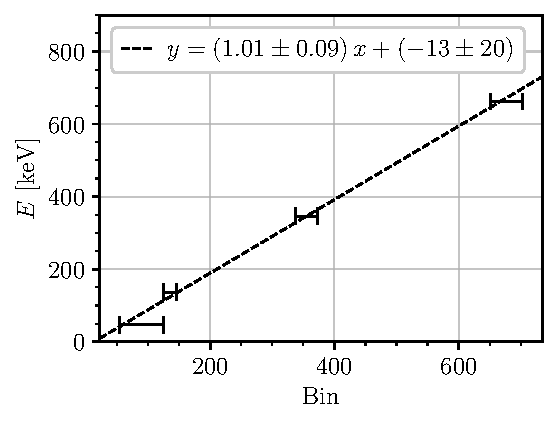
\includegraphics[scale=1]{figures/calibration_energy.pdf}
    \caption{Energy calibration of the spectrometer: known values of energies 
    versus the channel to which they were assigned by the MCA.}
    \label{fig:calibration_energy}
\end{figure}

Once the calibration was performed, it was possible to draw the $\gamma$ spectra 
of the four sources, as depicted in Figure \ref{fig:gamma_spectra}.
Comparing with the decay schemes, their $\gamma$ peaks were identified,
as well as the other contributions detailed in Section \ref{sec:spectrum}
the parasite contributions coming from the lead used to collimate 
the $\gamma$ rays (marked Pb), visible in the \cesium and \hafnium spectra, 
and the Compton edge, which appears most notably in the \cesium 
and the \lead spectra.
As expected (or detailed in Section \ref{sec:separation}), the $\gamma_2$ and $\gamma_3$ peaks of \cobalt are not distinguishable, due to blabla.
Also, only one $\gamma$ peak was detected for \hafnium, DETAIL.

\begin{figure}[htbp]
    \centering
    \begin{subfigure}{0.495\textwidth}
        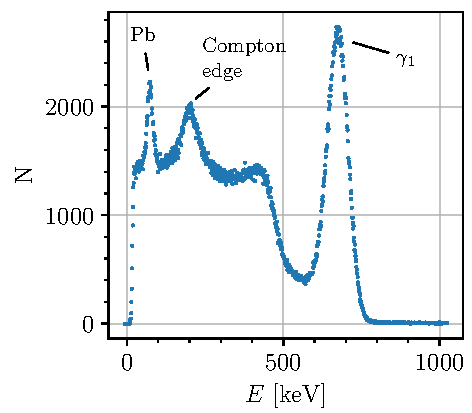
\includegraphics[scale=1]{figures/cs137_spectrum.pdf}
        \caption{}
    \end{subfigure}
    \hfill
    \begin{subfigure}{0.495\textwidth}
        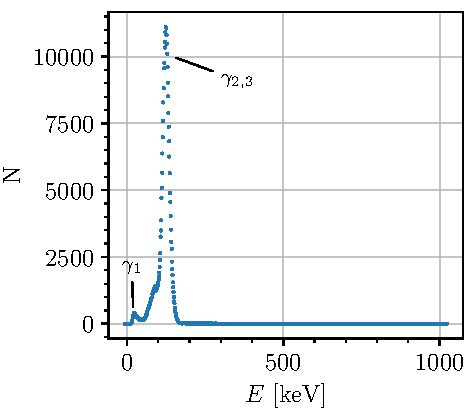
\includegraphics[scale=1]{figures/co57_spectrum.pdf}
        \caption{}
    \end{subfigure}
    \begin{subfigure}{0.495\textwidth}
        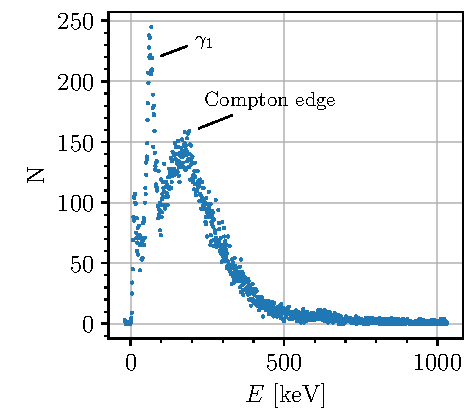
\includegraphics[scale=1]{figures/pb210_spectrum.pdf}
        \caption{}
    \end{subfigure}
    \hfill
    \begin{subfigure}{0.495\textwidth}
        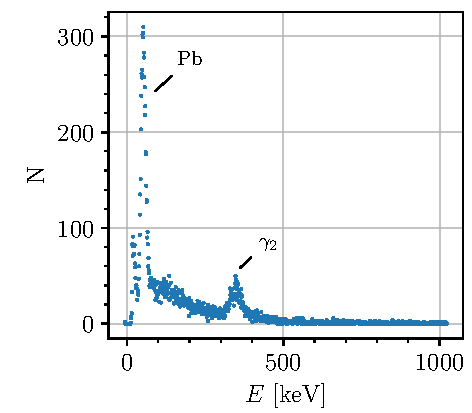
\includegraphics[scale=1]{figures/hf181_spectrum.pdf}
        \caption{}
    \end{subfigure}
    \caption{Gamma spectra of (a) $^{137}$Cs, (b) $^{57}$Co, (c) $^{210}$Pb, (d) $^{181}$Hf. \hl{METTRE LIGNE HORIZONTALE AU COMPTON PLATEAU}}
    \label{fig:gamma_spectra}
\end{figure}


\subsection{Statistics}
It was discussed in Section \ref{sec:statistics} that the number of desintegrations detected 
in a fixed interval of time follows a Poisson distribution, which tends to 
a gaussian distribution for a high mean.
To test these assumptions, two sets of measures were taken, using the MCA in MCS mode: 
the first ("lowmean") with a dwell time of $3$ ms, which gave an average of $m = 2.27$ desintegrations per interval, 
and the second ("highmean") with a dwell time of $300$ ms, with an average of $m = 228.10$.
Both were compared through Pearson's $\chi^2$ test 
with a Poisson distribution of parameter $\lambda = m$ 
and a gaussian distribution of mean $m$ and standard variation $\sqrt{m}$.
These test distributions are depicted in Figure \ref{fig:statistical_tests} with
the respective data sets
and the results of the statistical tests are summarised in Table \ref{tab:statistical_tests}.
%
\begin{figure}[htbp]
    \centering
    \begin{subfigure}{0.495\textwidth}
        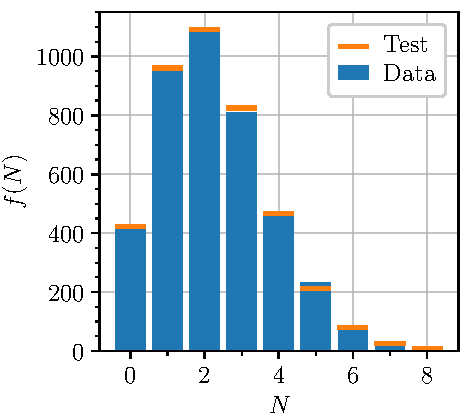
\includegraphics[scale=1]{figures/lowmean_poisson.pdf}
        \caption{}
    \end{subfigure}
    \hfill
    \begin{subfigure}{0.495\textwidth}
        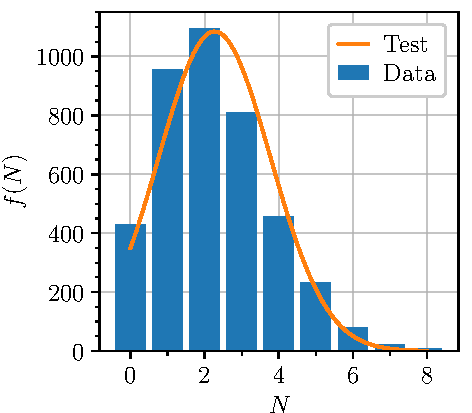
\includegraphics[scale=1]{figures/lowmean_gaussian.pdf}
        \caption{}
    \end{subfigure}
    \begin{subfigure}{0.495\textwidth}
        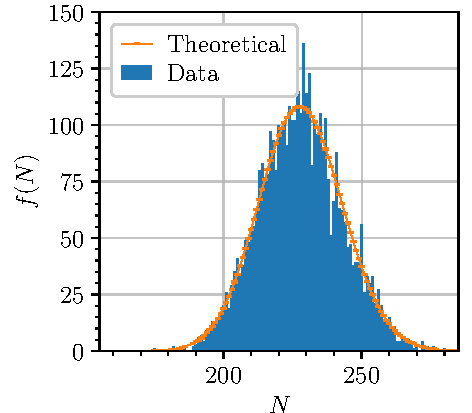
\includegraphics[scale=1]{figures/highmean_poisson.pdf}
        \caption{}
    \end{subfigure}
    \hfill
    \begin{subfigure}{0.495\textwidth}
        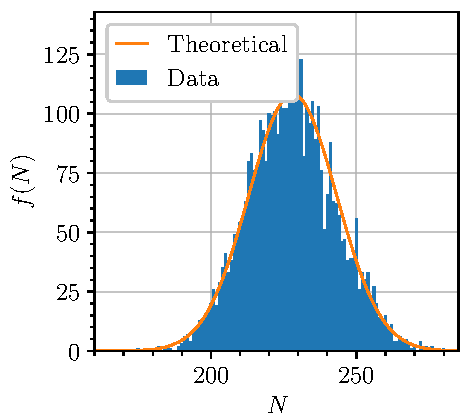
\includegraphics[scale=1]{figures/highmean_gaussian.pdf}
        \caption{}
    \end{subfigure}
    \caption{Frequencies of the number of desintegrations detected in a fixed interval of time, compared with test distributions: (a) lowmean and Poisson, (b) lowmean and gaussian, (c) highmean and Poisson, (d) highmean and gaussian \hl{Plus formel}}
    \label{fig:statistical_tests}
\end{figure}

\begin{table}[htbp]
    \centering
    \begin{tabular}{lllllll}
        \hline
        Data set & Mean & Test distribution & $\nu$ (or dof?) & $p$-value & Result \\
        \hline
        \multirow{2}{*}{Low mean} & \multirow{2}{*}{2.27} & Poisson & 8 & 0.86 & Accepted\\
        & & Gaussian & 7 & $5.7 \times 10^{-117}$ & Rejected \\
        \multirow{2}{*}{High mean} & \multirow{2}{*}{228.10} & Poisson & 91 & 0.38 & Accepted\\
        & & Gaussian & 90 & 0.26 & Accepted\\
        \hline
    \end{tabular}
    \caption{Results of the statistical tests on the distribution of the number of desintegrations detected in a fixed interval of time, carried out on two data sets of different mean.\hl{rendre plus clair} }
    \label{tab:statistical_tests}
\end{table}

\subsection{Attenuation in matter}
The study of the attenuation of $\gamma$ rays in matter was conducted using 
a sample of \cesium, a source more suited to the role than 
the others which were previously studied due to its higher activity\footnotemark.
Measures of the intensity of the radiation were taken for
different widths of aluminium and lead shielding applied 
between the source and the detector.
Figure \ref{fig:attenuation_coefficient} depicts the results obtained with 
the two materials:
the attenuation is exponential in nature, as described 
by Eq.\eqref{eq:attenuation_law}, and more effective using lead than aluminum.
The linear attenuation coefficient of each material was obtained by linear regression, yielding \mbox{$\mu = (0.20 \pm 0.01)$ \unit{\per\cm}} for aluminium
and \mbox{$\mu = (1.08 \pm 0.03)$ \unit{\per\cm}} for lead.\hl{$\mu_{\mathrm{Pb}}$?}
\begin{figure}[htbp]
    \centering
    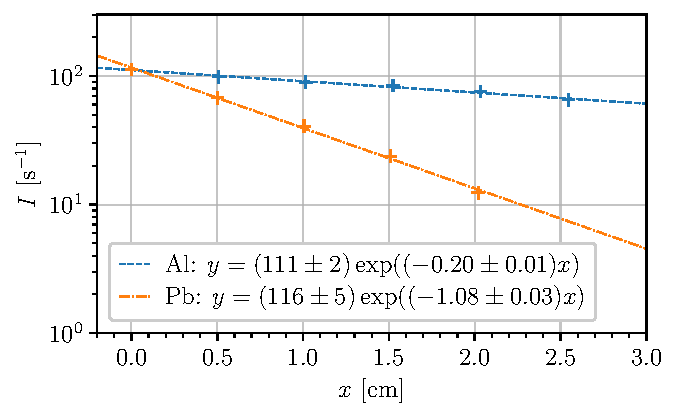
\includegraphics[scale=1]{figures/attenuation_coefficient.pdf}
    \caption{Radiation attenuation through Aluminum (Al) and Lead (Pb). 
             The error bars were omitted in reason of their small relative size 
             (1\% on the intensity and $1$ $\mu$m on the thickness of the material).}
    \label{fig:attenuation_coefficient}
\end{figure}
\footnotetext{J'ai comme l'impression que je peux écrire une phrase meilleure,
je vais probablement avoir l'idée pendant que je nage ou sous la douche.}

\subsection{Activity of \cobalt}
The experimental setup for coincidence detection described in Section \ref{sec:coincidences} allows for the calculation
of the activity A (see \autoref{eq:activity}). \hl{RÉECRIRE}
However, it was first necessary to determine the time resolution $2\theta$ of 
the instrument.

To this end, BLABLA

\begin{figure}[htbp]
    \centering
    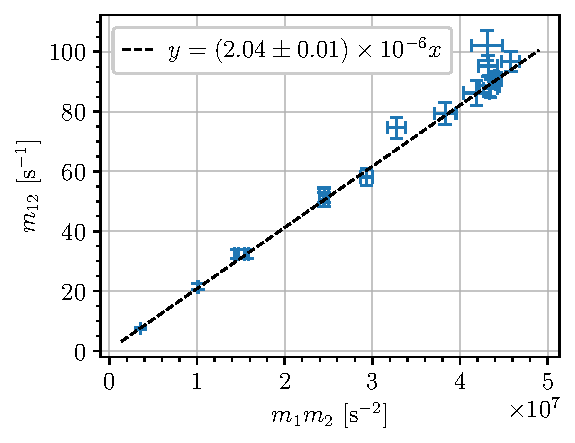
\includegraphics[scale=1]{figures/twotheta_cs137.pdf}
    \caption{\hl{Parler du cluster en haut à droite.}}
    \label{fig:twotheta_cs137}
\end{figure}


Having determined the resolution time of the coincidence selector, an activity $A= (4127 \pm 53)$ Bq was obtained.

\subsection{$\gamma_3$ spectrum}
\begin{figure}[htbp]
    \centering
    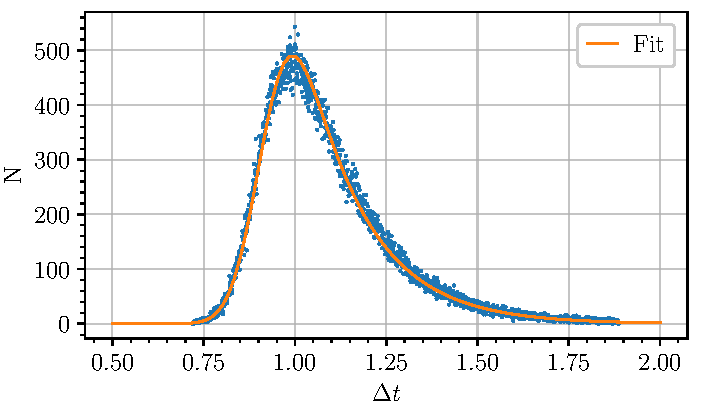
\includegraphics[scale=1]{figures/co57_halflife.pdf}
    \caption{}
    \label{fig:co57_gamma3_spectrum}
\end{figure}

\subsection{Half-life of 14.4 keV excited state}

\begin{figure}[h]
    \centering
    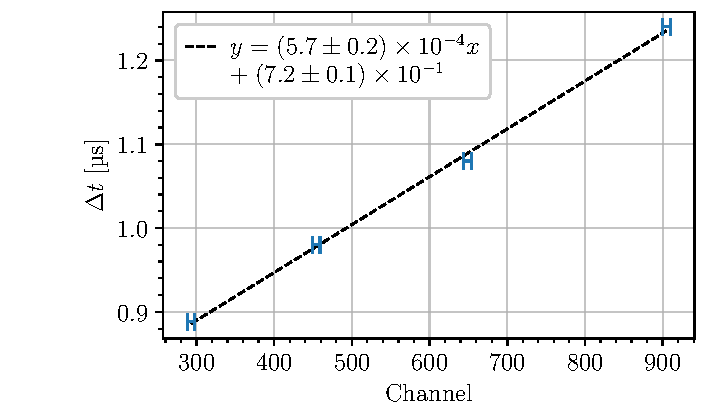
\includegraphics[width=0.6\textwidth]{figures/calibration_time_interval.pdf}    
    \caption{Calibration of channel to time for half-life measurement}
    \label{fig:calibration_halflife}
\end{figure}

\begin{figure}[h]
    \centering
    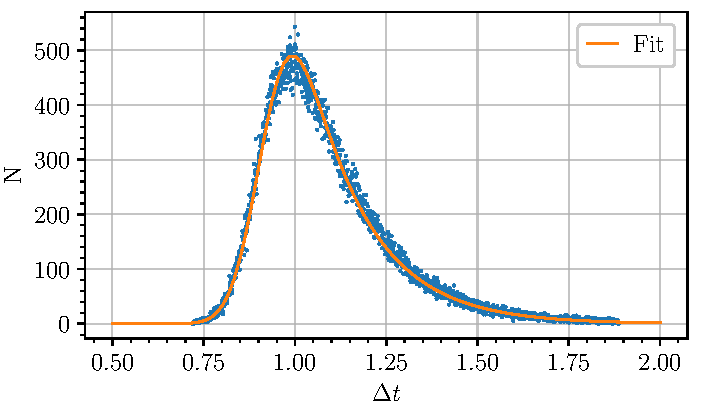
\includegraphics[width=0.6\textwidth]{figures/co57_halflife.pdf}    
    \caption{Measured delay between \(\gamma_2\) and \(\gamma_1\) signals}
    \label{fig:delay_gamma12}
\end{figure}

